\section{Model Overview and Architecture Details}
EmotionCNNet is a Convolutional Neural Network (CNN) designed for detecting facial expressions. The model was designed for image classification with an assumed input size of 48x48 pixels and three colour
channels (RGB). Convolutional layers are stacked with batch normalization and leaky ReLU activation. Each convolution layer has a kernel size of $ 4 * 4 $ with padding and stride of size 1. Max pooling technique was used for spatial reduction. The fully connected layer transforms learned features into class scores. A dropout layer (dropout) with a dropout rate of 0.5 is applied after the fourth convolutional layer. Dropout randomly sets a fraction of input units to zero during training, preventing overfitting by adding noise to the network.

\subsection*{Parallelism}
The \textit{nn.DataParallel} wrapper enables data parallelism, allowing the model to be trained on multiple GPUs simultaneously. This can significantly speed up the training process. The model is also moved to the GPU \textit{model.to(device)} for faster training if a GPU is available. Model parallelism allows computation to be distributed across available devices. \\

\noindent The model's performance on the validation set is monitored during training. If the model achieves better accuracy on the validation set subsequently, the model parameters are saved/updated. This helps prevent overfitting and provides the best-performing model.

\begin{table}[h!]
    \centering
    \begin{tabular}{ |p{4cm}|p{4cm}|p{4cm}| }
      \hline
      \textbf{Model} & \textbf{Convolution Layers} & \textbf{Kernel Size} \\
      \hline
      \textbf{Main Model} & 8 & 4\\
      \hline
      \textbf{Variant 1}  & 4 & 3\\
      \hline
      \textbf{Variant 2}  & 10 & 5\\
      \hline
    \end{tabular}
    \caption{Comparison of Models}
    \label{tab:model-comparison}
  \end{table}
 
  \subsubsection*{Variant 1}
  \noindent Max pooling is applied at specific convolution layers for reducing spacial dimensions resulting in a fully-connected layer of size 64 * 12 * 12.\\
  \subsubsection*{Variant 2}    
    \noindent Due to the increased kernel size, the padding had to be increased by a factor of 1. Max pooling was applied thrice to reduce the spatial dimensions, bringing it in line with a 2 * 2 kernel. The fully connnected layer is of size 512 * 6 * 6\\

\section{Training Process}
Following were the training hyperparameters set on the Main Model
\begin{itemize}
    \item \textbf{Number of Epochs}: 50
    \item \textbf{Learning Rate}: 0.01
    \item \textbf{Loss Function}: CrossEntropyLoss
    \item \textbf{Batch Size}: 64
    \item \textbf{Activation Function}: Leaky ReLU
    \item \textbf{Dropout}: Rate of 0.5
    \item \textbf{Device Placement}: GPU if available, else CPU
  \end{itemize}

  \begin{figure}[h!]
    \centering
    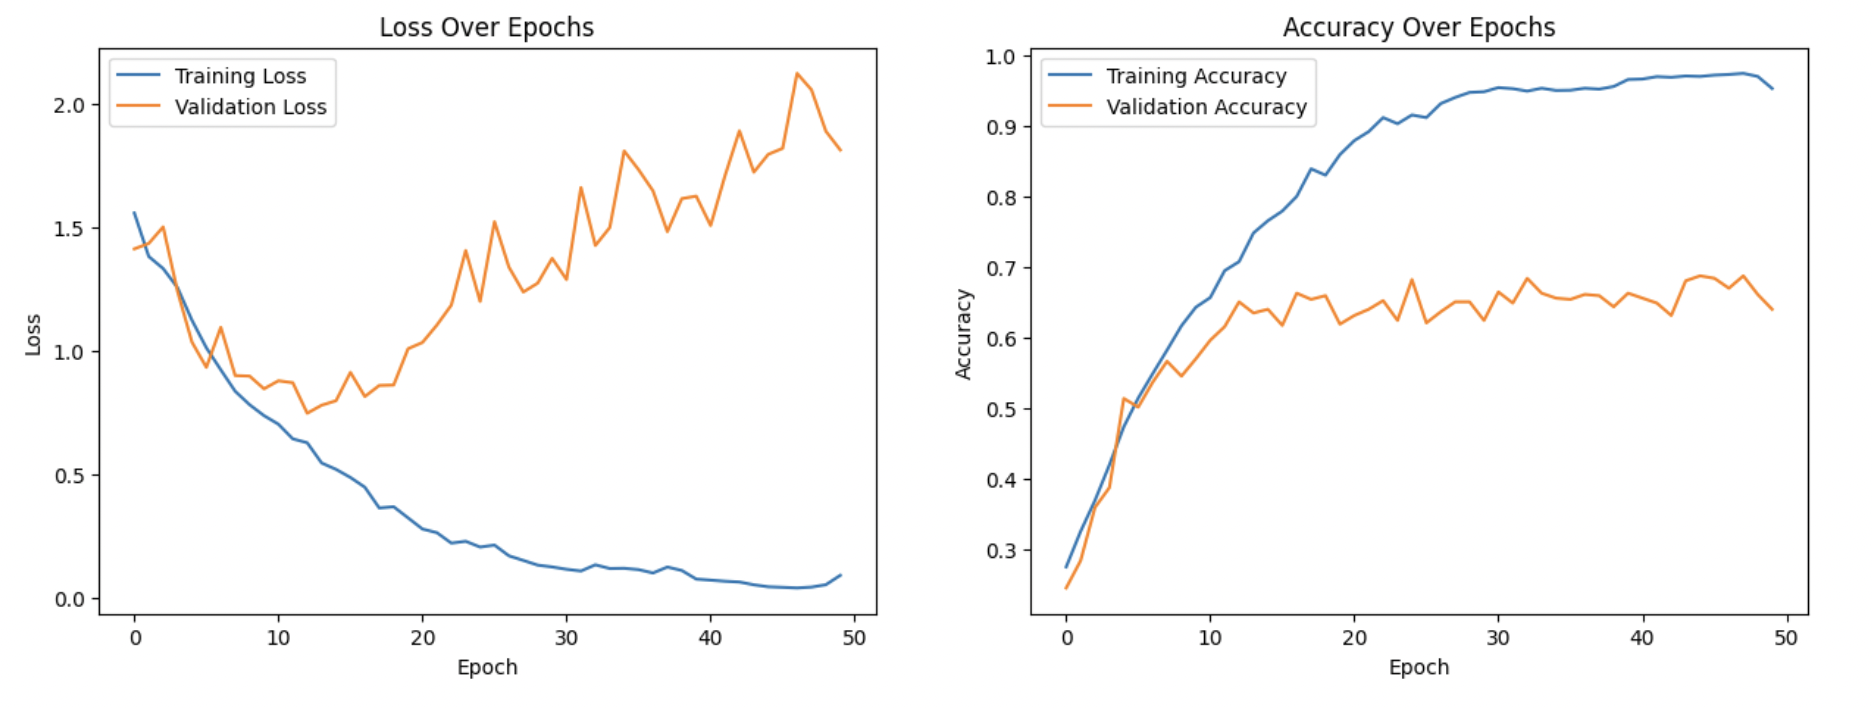
\includegraphics[width=0.9\textwidth, height=6cm]{resources/loss-acc-lg.png}
    \caption{Loss \& Accuracy after 50 Epochs}
  \end{figure}

\subsection*{Adam Optimizer and Loss Function}
The Adam optimizer \cite{AdamOptim} was used with a learning rate of 0.01. Adam combines the benefits of two other popular optimization algorithms—Adagrad and RMSprop—resulting in effective and adaptive learning rates. \\

\noindent Cross-Entropy Loss (\textit{nn.CrossEntropyLoss}) \cite{LossFunction} was used as the loss function. Cross-entropy loss is commonly used for multi-class classification problems.